\documentclass[12pt]{report}
\usepackage[numbers]{natbib}
\usepackage{graphicx}
\usepackage{float}
\usepackage{geometry}
 \geometry{
 a4paper,
 total={170mm,257mm},
 left=20mm,
 top=20mm,
 }


\begin{document}


\begin{titlepage}
   \begin{center}
       \vspace*{0.5cm}

       %---Write your title here----
      { \LARGE \textbf{ Leaf Disease Detection Using Machine Learning}}
	\vspace{1.5cm}

       \textit{A seminar report submitted in partial fulfilment of the requirements for the degree of}
            
       \vspace{0.2cm}

        {\large \textbf{MASTER OF SCIENCE}}

       \vspace{0.2cm}

        {\large \textbf{IN}}

          \vspace{0.2cm}
         
        %Write your domain here
        {\large \textbf{INFORMATION TECHNOLOGY}}
       %{\large \textbf{COMPUTER SCIENCE/INFORMATION TECHNOLOGY}}

                
       \vspace{2cm}
     
      \includegraphics[width=0.25\textwidth]{logo}
       
       \vspace{2cm}

       \textit{Submitted by}

       \vspace{0.2cm}
       \textbf{JENISH ALI BORAH (PS-211-811-0011)}
            
     \vspace{2cm}

       \textit{Supervised by}

       \vspace{0.2cm}
       \textbf{Dr. Hasin A. Ahmed}\\
       \textbf{Assistant Professor}

      \vspace{4cm}
      \textbf{\large DEPARTMENT OF COMPUTER SCIENCE}\\
       \textbf{\large GAUHATI UNIVERSITY, ASSAM}\\
      \textbf{\large 2022}

   \end{center}
\end{titlepage}


\clearpage
\pagenumbering{Roman} 



\vspace*{1cm}

\begin{center}


 \textbf{\large DEPARTMENT OF COMPUTER SCIENCE}

  \vspace{0.2cm}
 \textbf{\LARGE GAUHATI UNIVERSITY}\\
 {\large GUWAHATI - 781014}\\
 {\large ASSAM}

 \vspace{1cm}
     
 \includegraphics[width=0.15\textwidth]{logo}

 \vspace{2cm}

 \textbf{\large CERTIFICATE}

 \vspace{2cm}

\end{center}

This is to certify that the seminar report entitled \textbf{Leaf Disease Detection Using Machine Learning} submitted by \textbf{Jenish Ali Borah}, for partial fulfilment for the requirement of award of the degree of Master of Science in \textbf{Information Technology}, Gauhati University is a work carried out by him under my supervision and guidance.

To the best of my knowledge, the work has not been submitted to any other institute for the award of any other degree or diploma.

 \vspace{5cm}

\begin{tabular}{p{8cm} c}
Date:	 27-06-2023 &	Dr. Hasin A. Ahmed\\
Place: Gauhati University	&	Supervisor\\
	&	Assistant Professor\\
	&	Department of Computer Science\\
\end{tabular}


\pagebreak



\vspace*{2cm}

\begin{center}


  \textbf{\large DECLARATION}

  \vspace{5CM}

\end{center}

I hereby declare that the seminar report entitled \textbf{Leaf Disease Detection Using Machine Learning} has been compiled by me and
submitted in partial fulfilment for the requirement of award of the degree of \textbf{Master of Science in Information Technology}, Gauhati University. I also declare that any or all contents incorporated in
the report has not been submitted in any form for the award of any other degree of any other institute or university.

 \vspace{5cm}

\begin{tabular}{p{8cm} p{15cm} l}
Date: 27-06-2023	&	Jenish Ali Borah\\
Place: Gauhati University	&	Roll No.: PS-211-811-0011\\
	&	Programme: Information Technology\\
	&	Semester: Fourth Semester\\

\end{tabular}



\tableofcontents
\thispagestyle{empty}

\clearpage
\pagenumbering{arabic} 
\setcounter{page}{1}
\chapter{Introduction}
This is a header statement. This is a header statement. This is a header statement. This is a header statement. This is a header statement. This is a header statement. This is a header statement \citep{mahanta2008finding}. This is a header statement. This is a header statement. This is a header statement. This is a header statement. This is a header statement \citep{dutta2005qrock}. 
\section{Problem domain introduction}
This is a statement on problem. This is a statement on problem. This is a statement on problem. This is a statement on problem. This is a statement on problem. This is a statement on problem. This is a statement on problem. This is a statement on problem. This is a statement on problem. This is a statement on problem. This is a statement on problem. This is a statement on problem. This is a statement on problem. This is a statement on problem. This is a statement on problem. This is a statement on problem. 
\subsection{Problems in the domain}
This is a sample statement in the subsection. This is a sample statement in the subsection. This is a sample statement in the subsection. This is a sample statement in the subsection. This is a sample statement in the subsection. This is a sample statement in the subsection. This is a sample statement in the subsection. This is a sample statement in the subsection. This is a sample statement in the subsection. This is a sample statement in the subsection. This is a sample statement in the subsection. This is a sample statement in the subsection. This is a sample statement in the subsection. This is a sample statement in the subsection. This is a sample statement in the subsection.
\begin{figure}[H]
\label{figTiger}
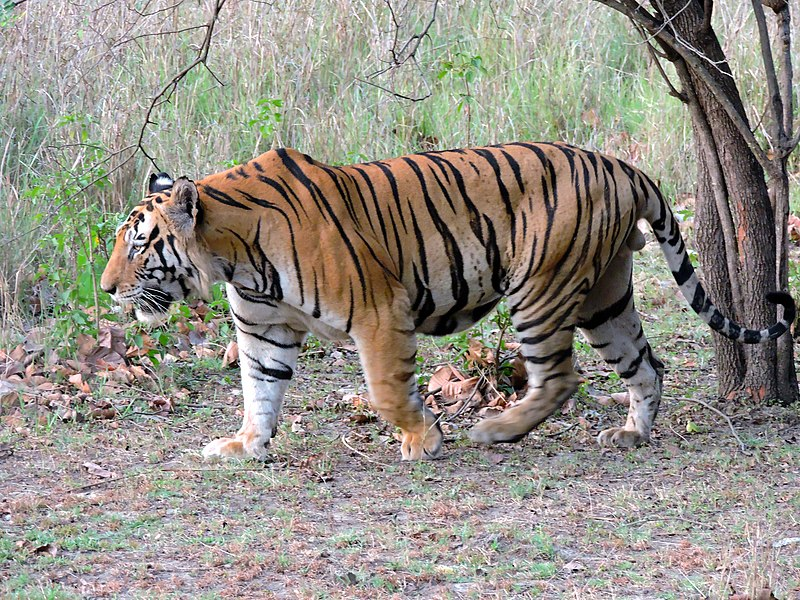
\includegraphics[width=8cm]{tiger.jpg}
\centering
\caption{Tiger (source: wikipedia)}
\end{figure} 
\section{Problem definition}
This is a statement on problem. This is a statement on problem. This is a statement on problem. This is a statement on problem. This is a statement on problem. This is a statement on problem. This is a statement on problem. This is a statement on problem. This is a statement on problem. This is a statement on problem. This is a statement on problem. This is a statement on problem. This is a statement on problem. This is a statement on problem. This is a statement on problem. This is a statement on problem. 
\section{Delimitations of the current problem solution}
This is a statement on problem. This is a statement on problem. This is a statement on problem. This is a statement on problem. This is a statement on problem. This is a statement on problem. This is a statement on problem. This is a statement on problem. This is a statement on problem. This is a statement on problem. This is a statement on problem. This is a statement on problem. This is a statement on problem. This is a statement on problem. This is a statement on problem. This is a statement on problem. 

\chapter{Literature Review}
This a sample statement in literature review. This a sample statement in literature review. This a sample statement in literature review. This a sample statement in literature review. This a sample statement in literature review. This a sample statement in literature review. This a sample statement in literature review. This a sample statement in literature review. This a sample statement in literature review. This a sample statement in literature review. This a sample statement in literature review. This a sample statement in literature review. 
\section{Existing Methods}
Thsi is a sample statement in Existing Methods. This a sample statement in literature review. This a sample statement in literature review. This a sample statement in literature review. This a sample statement in literature review. This a sample statement in literature review. This a sample statement in literature review. 

\section{Comparison of Existing Methods}
This is a sample statement in Existing Methods. This a sample statement in literature review. This a sample statement in literature review. This a sample statement in literature review. This a sample statement in literature review. This a sample statement in literature review. This a sample statement in literature review. 

\section{Limitations of Existing Methods}
Thsi is a sample statement in Existing Methods. This a sample statement in literature review. This a sample statement in literature review. This a sample statement in literature review. This a sample statement in literature review. This a sample statement in literature review. This a sample statement in literature review. 

\chapter{Proposed Method}
This is a sample header statement. This is a sample header statement. This is a sample header statement. This is a sample header statement. This is a sample header statement. This is a sample header statement. This is a sample header statement. This is a sample header statement. This is a sample header statement. This is a sample header statement. This is a sample header statement. This is a sample header statement. This is a sample header statement. This is a sample header statement. 

\section{Proposed Algorithm}
This is a sample statement. This is a sample statement.This is a sample statement.This is a sample statement.This is a sample statement.This is a sample statement.This is a sample statement.This is a sample statement.This is a sample statement.This is a sample statement.This is a sample statement.This is a sample statement.

\section{Comparison with the Existing Technique}
This is a sample statement. This is a sample statement.This is a sample statement.This is a sample statement.This is a sample statement.This is a sample statement.This is a sample statement.This is a sample statement.This is a sample statement.This is a sample statement.This is a sample statement.This is a sample statement. This is reported in Figure \ref{figTiger}.


\chapter{Implementation}
This is a sample $a<b$ header statement. This is a sample header statement. This is a sample header statement. This is a sample header statement. This is a sample header statement. This is a sample header statement. This is a sample header statement. This is a sample header statement. This is a sample header statement. This is a sample header statement. This is a sample header statement. This is a sample header statement. This is a sample header statement. This is a sample header statement. 


\section{Environment Used}
This is a sample statement. This is a sample statement.This is a sample statement.This is a sample statement.This is a sample statement.This is a sample statement.This is a sample statement.This is a sample statement.This is a sample statement.This is a sample statement.This is a sample statement.This is a sample statement.

\section{Tools Used}
This is a sample statement. This is a sample statement.This is a sample statement.This is a sample statement.This is a sample statement.This is a sample statement.This is a sample statement.This is a sample statement.This is a sample statement.This is a sample statement.This is a sample statement.This is a sample statement.

\chapter{Results and Discussion}
This is a sample header statement. This is a sample header statement. This is a sample header statement. This is a sample header statement. This is a sample header statement. This is a sample header statement. This is a sample header statement. This is a sample header statement. This is a sample header statement. This is a sample header statement. This is a sample header statement. This is a sample header statement. This is a sample header statement. This is a sample header statement. 

\section{Datasets Used}
This is a sample statement. This is a sample statement.This is a sample statement.This is a sample statement.This is a sample statement.This is a sample statement.This is a sample statement.This is a sample statement.This is a sample statement.This is a sample statement.This is a sample statement.This is a sample statement.

\section{Empirical Analysis}
Result is reported in Table \ref{sampletable}. This is a sample statement. This is a sample statement.This is a sample statement.This is a sample statement.This is a sample statement.This is a sample statement.This is a sample statement.This is a sample statement.This is a sample statement.This is a sample statement.This is a sample statement.This is a sample statement.

\begin{table}
\label{sampletable}
\caption{Table reporting Empirical Result}
\centering
\begin{tabular}{ |l|l| }
  \hline
  \multicolumn{2}{|c|}{Team sheet} \\
  \hline
  GK & Paul Robinson \\
  LB & Lucas Radebe \\
  DC & Michael Duberry \\
  DC & Dominic Matteo \\
  RB & Dider Domi \\
  MC & David Batty \\
  MC & Eirik Bakke \\
  MC & Jody Morris \\
  FW & Jamie McMaster \\
  ST & Alan Smith \\
  ST & Mark Viduka \\
  \hline
\end{tabular}
\end{table}

\chapter{Conclusion}
This is a sample header statement. This is a sample header statement. This is a sample header statement. This is a sample header statement. This is a sample header statement. This is a sample header statement. This is a sample header statement. This is a sample header statement. This is a sample header statement. This is a sample header statement. This is a sample header statement. This is a sample header statement. This is a sample header statement. This is a sample header statement. 

\section{Concluding Remarks}
This is a sample statement. This is a sample statement.This is a sample statement.This is a sample statement.This is a sample statement.This is a sample statement.This is a sample statement.This is a sample statement.This is a sample statement.This is a sample statement.This is a sample statement.This is a sample statement.

\section{Future Work}
This is a sample statement. This is a sample statement.This is a sample statement.This is a sample statement.This is a sample statement.This is a sample statement.This is a sample statement.This is a sample statement.This is a sample statement.This is a sample statement.This is a sample statement.This is a sample statement.

\bibliography{refs}
\bibliographystyle{apalike} 
 

\end{document}